% Preamble
\documentclass[12pt,a4paper]{article}
\usepackage{enumerate} 	
\usepackage{setspace}						
\usepackage{authblk}	
\usepackage{graphicx} 	
%\usepackage[nomarkers, nolists]{endfloat} 
\usepackage{pdflscape}	
\usepackage{mathtools}	
\usepackage[osf]{mathpazo} 
\usepackage{lineno} 
\usepackage{ms}    	
\usepackage{hyperref}
\usepackage[round]{natbib} 
\usepackage{setspace}

\setcounter{secnumdepth}{0} 
\raggedright 			
\pagenumbering{arabic}	
\linenumbers


% First order headings upper case bold
\usepackage{titlesec}
\titleformat*{\section}{\small\bfseries\uppercase}

% Second order headings normal case italics
\titleformat*{\subsection}{\small\itshape}

% Third order, italics, paragraph style
\titleformat*{\paragraph}{\small\itshape}


% lists - arabic in (1; (2); (3) .


% Title page information

\title{Time for a rethink: disparity-through-time}
%TG: Great title first part! How about changing the other part to 
%Time for a rethink: different ways of slicing through the stratigraphic cake leads to different disparity through time results.

\author{
	Thomas Guillerme$^{1*}$ and Natalie Cooper$^{2}$
}
%TG: authorship-wise it's up to you, in the end, since it's just the two of us, I think it really doesn't matter (i.e. it's still gonna be Cooper Guillerme or Guillerme Cooper), I'll hopefully will have a couple of first author papers coming up for 2018 so up to you if you want one as well.

\date{}

\affiliation{\noindent{\footnotesize
	$^1$School of Biological Sciences, University of Queensland, St. Lucia, Queensland, Australia.\\
	$^2$Department of Life Sciences, Natural History Museum, Cromwell Road, London, SW7 5BD, UK. natalie.cooper@nhm.ac.uk}\\
	$^*$Corresponding author\\}

\vfill

\runninghead{Time sub-samples in disparity-through-time analyses}
\keywords{time bin, time slice, disparity} 
% up to 6

\begin{document}

\mstitlepage
\parindent = 1.5em
\addtolength{\parskip}{.3em}

\section{Abstract}
% 300 words max
	

\newpage
\raggedright
\doublespacing
\setlength{\parindent}{1cm}

\section{Introduction}
%TG: Plan idea
%TG: §1: disparity-through-time really cool and well used
%TG: §2: caveats with both disparity and through-time part
%TG: §3: specific ways to look through-time and their problems
%TG: §4: our kind of solution

Disparity-through-time analyes are common in palaeontology \citep{Foote01071994}.
They reveal how the morphological diversity of clades has changed through time, and allow us to make inferences about the breadth of ecological niches extinct taxa occupied \citep{foote1997evolution}.
Results from disparity-through-time studies also provide insights into the ecological impacts of mass extinctions, competitive replacements, and the drivers of morphological evolution \citep{Brusatte12092008,Foote29111996,friedmanexplosive2010}.
Unfortunately, the way we perform these analyses may have profound effects on our conclusions.

% However, our methods for analysing diversity-through-time have not changed all that much in the XX years they have been popular. %TG: small caveat on that after litterature search for the disparity review paper: disparity-through-time analysis have not changed much since Foote 1992, Foote and Gould 1992 and Briggs et al. 1992 in the classic palaeobiology appro,ach...
%TG: However to not piss of people, there were several attempts to "rationalise" (Wills 2001), test (Ciampaglio 2001) and expand (Pavlinov 2011 and Gerber et al 2011) namely with univariate approaches and "dtt" analysis (Harmon et al 2003).
%TG: One of the critisisms from one of the rude reviews was this idea that age of popular method has nothing to do with its performance, by nuancing this sentence we can basically say: yeah, some people have made great advances and proposed great ideas for CORRECTING ERRORS in the methods from the 90s but somehow everybody have ignored them (in palaeobiology).
% NC: OK so lets save ourselves some pain and not mention this at all and save it all for the bitching in the review paper!!!
% TG: agree!

Disparity-through-time analyes have two main analysis components: calculating disparity, and creating time sub-samples of the data. 
Here we focus on the latter.
The nature of disparity (it is a diversity metric), means it cannot be calculated using just one individual, so some way of subsetting taxa is required.
Changes in disparity-through-time are generally investigated by calculating the disparity of taxa present during specific time intervals or time bins \citep[e.g][]{cisneros2010,prentice2011,Hughes20082013,hopkinsdecoupling2013,bentonmodels2014,bensonfaunal2014}.
These time bins are usually defined based on stratigraphy \citep[e.g.][]{cisneros2010,prentice2011,Hughes20082013,bentonmodels2014} but can also be arbitrarily chosen time bins of equal duration \citep{Butler2012,hopkinsdecoupling2013,bensonfaunal2014}.
However, this approach has several limitations.

First, time bins defined by stratigraphy are not of equal size, biasing higher disparity towards longer stratigraphic periods. 
This can be dealt with using rarefaction, i.e. repeating the analysis using the smallest number of taxa present in any bin as the number of sampled taxa in each bin. 
This can, however, lead to very large confidence intervals when there are stratigraphic periods with very few species.
Other studies split large time bins so they are of roughly equal size, but this is often an \textit{ad hoc} procedure that can introduce more bias depending on where bins are split.
Second, all time binning approaches (whether bins are equally sized or not) assume that characters of taxa evolve following a punctuated equilibrium model, because disparity is only estimated once for each interval resulting in all changes in disparity occurring \textit{between} intervals, rather than also allowing for gradual changes \textit{within} intervals \citep{Hunt21042015}.
Finally, time bin analyses are often limited by the number of taxa in each bin.
If there are insufficient taxa in a time bin, disparity cannot be calculated, so further analyses, e.g. correlations of disparity with hypothesised drivers of morphological evolution, are not possible.

To address these issues, we propose a ``time-slicing'' approach that takes advantage of the wealth of paleontological datasets which now have associated phylogenies. 
Time-slicing uses a phylogenetic tree and considers subsets of taxa at specific equidistant points in time, as opposed to considering subsets of taxa between two points in time.
This results in even-sampling across time and permits us to define the underlying model of character evolution (punctuated or gradual).  
Time-slicing also includes any element present in the phylogeny (branches, nodes and tips) at the time slice in question as part of the disparity calculation.
This allows us to measure disparity at time points where there are no terminal taxa, and increases the sample size at each time point, making downstream analyses of the drivers of disparity much more feasible.

Here we present our time-slicing methods using four datasets taken from the literature.
We calculate disparity-through-time for each dataset using a range of time binning and time-slicing methods, and then compare these approaches with respect to the relative disparities calculated, but also with how the different approaches influence biological conclusions. We find that XXX

\section{Materials and Methods}
\subsection{Overview}
\label{overview-section}
To test the different time sub-sampling methods, we followed the protocol below (Figure \ref{datasets}). 
All the code needed to reproduce these analyses (along with detailed instructions) is provided on GitHub (https://github.com/nhcooper123/time-slice). 

https://rawgit.com/TGuillerme/dispRity/master/inst/gitbook/_book/details-of-specific-functions.html#time-slicing

% NC: might move this to the NHM github account
% TG: why that? It'll be just extra hassle no?

% Add overview figure
%TG: This is a first draft of the figure and its caption. Tell me what you think.

  \begin{figure}[!htbp]
    \centering
    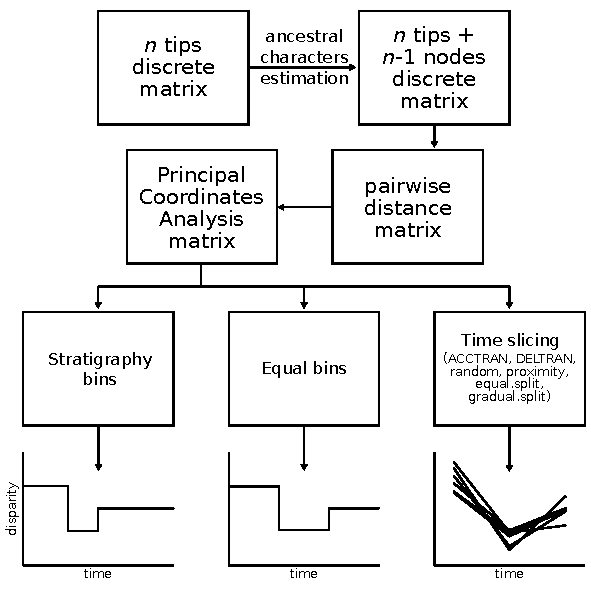
\includegraphics[width=1\linewidth, height=1\textheight, keepaspectratio]{outlinesvg.pdf}
    \caption[caption title]
    {Outline of the disparity-through-time pipeline applied to each data set: 1) we used ancestral characters estimation to infer nodal character states, 2) we measured the pairwise Gower distance between the tips and nodal characters, 3) we ordinated the distance matrix using a PCoA, 4) we split that matrix using stratigraphy bins, equal bins and the time slice method, 5) we measured disparity through time for each of these methods.}
    \label{overview}
  \end{figure}

\subsection{Example datasets}
\label{datasets}
To test the different time binning/slicing methods we selected four datasets: a mammal dataset from \cite{beckancient2014}, two theropod datasets from \cite{brusatte2014gradual} and \cite{bapst2016topology}, and a crinoid dataset from \cite{wright2017bayesian}.
Table \ref{table:datasets} and appendix ??? provide more details. % add appendix details
Each dataset consists of first and last occurrence dates for all taxa, a matrix of morphological characters in NEXUS format, and a time-scaled phylogeny. 
These datasets are freely available with their accompanying papers (Table \ref{table:datasets}), but for reproducibility purposes we also provide the data we used on GitHub (https://github.com/nhcooper123/time-slice/data).

% Dataset details table
\begin{landscape}
  % latex table generated in R 3.4.3 by xtable 1.8-2 package
% Wed Dec 20 13:12:18 2017
\begin{table}[!htbp]
\caption{Details of the datasets used in this study. Age ranges are root time to most recent tip taxon.} 
\centering
\begin{tabular}{lcccc}
  \hline
 & \textbf{Beck2014} & \textbf{Brusatte2014} & \textbf{Bapst2016} & \textbf{Wright2017} \\ 
  \hline
Group & mammals & theropods & theropods & crinoids \\ 
  \# taxa & 106 & 152 &  89 &  42 \\ 
  \# characters & 421 & 853 & 374 &  87 \\ 
  Age range (MYA) & 171.8 - 0 & 168.5 - 66 & 207.2 - 66 & 485.4 - 372.2 \\ 
  Mass extinction (MYA) & 66 (K-Pg) & NA & NA & 443 (O-S) \\ 
  Reference & \cite{beckancient2014} & \cite{brusatte2014gradual} & \cite{bapst2016topology} & \cite{wright2017bayesian} \\ 
  Data reference &  \cite{beckancient2014} & \cite{dryad_84t75} & \cite{dryad_n2g80} &  \cite{dryad_6hb7j} \\ 
   \hline
\end{tabular}
\label{table:datasets}  
\end{table}
 
  \label{table:datasets}  
\end{landscape}

\subsection{Preparing the data for disparity-through-time analysis}

\paragraph{Estimating ancestral character states.}
\label{ace}
For each dataset we used the re-rooting method \citep{Yang01121995,Garland2000} to get Maximum Likelihood estimates of the ancestral states for each character at every node in the phylogeny, using the \texttt{rerootingMethod} function from the \texttt{R} package \texttt{phytools} version 0.6-44 \citep{phytools,R}.
Where there were missing character data for a taxon we followed the method of \cite{Claddis} and treated missing data as any possible observed state for each character.
For example, if a character had two observed states ($0$ and $1$) across all taxa, we attributed the multi-state ``$0$\&$1$" value to the taxon with missing data, representing an equal probability of being either $0$ or $1$.
This allows the ancestral node of a taxon with missing data to be estimated with no assumptions other than that the taxon has one of the observed character states.
To prevent poor ancestral state reconstructions from biasing our results, especially when a lot of error is associated with the reconstruction, we only included ancestral state reconstructions with a scaled Likelihood $\geq$ $0.95$.
Ancestral state reconstructions with scaled Likelihoods below this threshold were recoded as missing data (``?'').

\paragraph{Building cladisto-spaces.} 
To explore disparity-through-time in our datasets we used a cladisto-space approach \citep[e.g.][]{Foote01071994,Foote29111996,Wesley-Hunt2005,Brusatte12092008,friedmanexplosive2010,toljagictriassic-jurassic2013,Hughes20082013}.
This approach is similar to constructing a morphospace based on continuous morphological data \citep[e.g.][]{friedmanexplosive2010}, except a cladisto-space is an approximation of the morphospace based on cladistic data (i.e. the discrete morphological characters used to build a phylogenetic tree).
Mathematically, a cladisto-space is an $n$ dimensional object that summarises the cladistic distances between the taxa present in a cladistic matrix.
Although empirically inter-taxon distances are the same in a morphospace or a cladisto-space \citep{foth2012different,hetherington2015cladistic}, we prefer the term cladisto-space to make it clear that this space is estimated using cladistic data and not morphometric data.

\paragraph{Constructing distance matrices.}
To estimate the cladisto-spaces for each of our datasets we first constructed pairwise distance matrices of length $k$, where $k$ is the total number of tips and nodes in the dataset.
We calculated the $k$$\times$$k$ distances using the Gower distance \citep{Gower71}, i.e. the Euclidean distance between two taxa divided by the number of shared characters. 
This allows us to correct for distances between two taxa that share many characters and could be closer to each other than to taxa with fewer characters in common (i.e. because some pairs of taxa share more characters in common than others, they are more likely to be similar).
For cladistic matrices, using this corrected distance is preferable to the raw Euclidean distance because of its ability to deal with discrete or/and ordinated characters as well as with missing data \citep{anderson2012using}.
However, the Gower distance cannot calculate distances when taxa have no overlapping data.
Therefore, we used the \texttt{TrimMorphDistMatrix} function from the \texttt{Claddis} \texttt{R} package \citep{Claddis} to remove pairs of taxa with no cladistic characters in common.
This led to us removing nine taxa from the \cite{bapst2016topology} dataset, and 19 from the \cite{brusatte2014gradual} dataset, but none from the other two datasets (see appendix for details of which species). 
% add appendix details

\paragraph{Ordination.}
After constructing our distance matrices we transformed them using classical multidimensional scaling \citep[MDS;][]{torgerson1965multidimensional,GOWER01121966,cailliez1983analytical}.
This method (also referred to as PCO; e.g. \citealt{Brusatte2015}; or PCoA; e.g. \citealt{paradisape:2004}) is an eigen decomposition of the distance matrix.
Because we used Gower distances instead of raw Euclidean distances, negative eigenvalues can be calculated.
To avoid this problem, we first transformed the distance matrices by applying the Cailliez correction \citep{cailliez1983analytical} which adds a constant $c^*$ to the values in a distance matrix (apart from the diagonal) so that all the Gower distances become Euclidean ($d_{Gower}+c^*=d_{Euclidean}$; \citealt{cailliez1983analytical}). 
We were then able to extract $n$ eigenvectors for each matrix (representing the $n$ dimensions of the cladisto-space) where $n$ is equal to $k-2$, i.e. the number of taxa in the matrix ($k$) minus the last two eigenvectors that are always null after applying the Cailliez correction.
Contrary to previous studies \citep[e.g][]{brusatte50,cisneros2010,prentice2011,anderson2012using,Hughes20082013,bentonmodels2014}, we use all $n$ dimensions of our cladisto-spaces and not a sub-sample representing the majority of the variance in the distance matrix (e.g. selecting only $m$ dimensions that represent up to 90\% of the variance in the distance matrix; \citealt{Brusatte12092008,toljagictriassic-jurassic2013}).

Note that our cladisto-spaces represent an ordination of all possible morphologies coded in each study through time.
It is unlikely that all morphologies will co-occur at each time point, therefore, the disparity of the whole cladisto-space is expected to be greater than the disparity at any specific point in time.

\subsection{Disparity-through-time analyses}

\paragraph{Calculating disparity.}
\label{disparity_calc}
Disparity can be calculated in many different ways \citep[e.g.][]{Wills1994,Ciampaglio2004,thorneresetting2011,hopkinsdecoupling2013,huang2015origins}, however most studies estimate disparity using four metrics: the sum and products of ranges and variances, each of which gives a slightly different estimate of how the data fits within the cladisto-space \citep{Foote01071994,Wills1994,brusatte50,Brusatte12092008,cisneros2010,thorneresetting2011,prentice2011,brusattedinosaur2012,toljagictriassic-jurassic2013,ruta2013,bentonmodels2014,bensonfaunal2014}.
However, these metrics have limitations. 
First, the range metrics are affected by the uneven sampling of the fossil record \citep{Butler2012}.
Second, because we include all $n$ dimensions in the analysis (see above), the products of ranges and variances will tend towards zero since the scores of the last dimension are usually really close to zero themselves. 
We therefore use the sum of variances metric to estimate disparity here.
Note that there are still statistical issues with this metric, but for the purposes of comparison with previous work we want to use a standard metric for these analyses.

\paragraph{Time sub-sampling} 
\label{time_sub-samples}

To estimate disparity-through-time we first need to split the data into time sub-samples.
Here we use three time sub-sampling methods.

\begin{enumerate}
  \item Stratigraphic time bins. This is the traditional method, where all the taxa within each stratigraphic period are included in the disparity calculation. This often leads to bins of unequal duration. Here we use stratigraphic ages and epochs.
  \item Equally sized time bins. This is another commonly used method, where the time frame of interest is split into equally sized time bins, then all the taxa within each time bin are included in the disparity calculation. 
  \item Time-slicing. We describe this in more detail below, but in brief, time-slicing uses a phylogeny, and rather than binning the data, it takes slices through a phylogeny and includes all the taxa and nodes in that slice within the disparity calculation. 
\end{enumerate}  

\paragraph{Time-slicing} 
\label{time_slicing}
The ``time-slicing'' approach considers subsets of taxa in the cladisto-space at specific equidistant points in time, as opposed to considering subsets of taxa between two points in time.
This results in even-sampling of the cladisto-space across time and allows us to use different underlying models of character evolution (punctuated or gradual). 

In practice, time-slicing considers the disparity of any element present in the phylogeny (branches, nodes and tips) at any point in time.
When the phylogenetic elements are nodes or tips, the ordination scores for the nodes (estimated using ancestral state reconstruction as described above) or tips are directly used for calculating disparity.
When the phylogenetic elements are branches we choose the ordination score for the branch using one of two evolutionary models:

%TG: Not sure if it's the "egeinvector" score or the "eigen" score. I think there's a trick in naming them depending on how the algorithm does the transformation (soemthing with using eigenvalues or eigenvectors). I call it ordination score for now.


\begin{enumerate}

    \item{\textbf{Punctuated evolution.}} 
    This model selects the ordination score from either the ancestral node or the descendant node/tip of the branch regardless of the position of the slice along the branch. 
    Similarly to the time bin approach, this reflects a model of punctuated evolution where changes in disparity occur either at the start or at the end of a branch over a relatively short time period, and clades undergo long periods of stasis during their evolution \citep{Gould1977,Hunt20112007}.
    We apply this model in four ways: 

    \begin{enumerate}[(i)]

      \item The ``acctran'' model, always selecting the ordination score of the ancestral node of the branch.
      \item The ``deltran'' model, always selecting the ordination score of the descendant node/tip of the branch.
      \item The ``random'' model, randomly selecting the ordination score of either the ancestor or the descendant of the branch.
      \item The ``proximity'' model, selecting the ordination score of the ancestor if the slice occurs in the first half of the branch, and the descendant if the slice occurs in the second half of the branch.

    \end{enumerate}

    The two first models assume that changes always occur early (ACCelerated TRANsition) or late along the branches (DELayed TRANsition).
    The third model makes neither assumption and simply selects data from the ancestor or the descendant at random, and the fourth bases the selection of either the ancestor or the descendant on where the slice occurs along the branch.
    The punctuated models only select either the ordination score from the ancestor and the descendant once in the whole disparity analysis.
    For example, if using the ``random'' model, if the data of the ancestor has been randomly chosen, only this data will be used during the bootstrapping (see below) and for the disparity calculation.
    
    \item{\textbf{Gradual evolution.}}
    Unlike the punctuated models, the following models do not select the ordination score of either the ancestor or the descendant but associate a probability to both.
    This reflects a model of gradual evolution where changes in disparity are gradual and cumulative along the branch.

    \begin{enumerate}[(i)]
    \setcounter{enumii}{4}
      \item The ``equal splits'' model (probabilistic), selects the ordination score from both the ancestor and the descendant with an equal probability
          \begin{equation}
          p(\text{ancestor}) = p(\text{descendant}) = 0.5
          \end{equation}

    \item The ``gradual splits'' model (probabilistic), selects the ordination score from both the ancestor and the descendant with a probability function of the distance between the nodes/tips and the slice.
    % NC: I'm unsure what you mean here: "the distance between the slice." Do you mean the branch length, the interval between slices, or the distance between the slice and the node?
    %TG: I've clarified as above. Tell me if it's clearer. In my words: the distance between the slice and the node, like you illustrate in your presentation (nicely done by the way!)
          \begin{equation}
              p(\text{ancestor}) = \frac{d(\text{ancestor},\text{slice})}{d(\text{ancestor},\text{descendant})}
          \end{equation}
          \begin{equation}
              p(\text{descendant}) = 1 - p(\text{ancestor})
          \end{equation}
    \noindent Where $d(x,y)$ is the distance measured as branch length.
    \end{enumerate}

    In these models, the ordination scores of both the ancestor and descendant contribute to the disparity calculation.
    For example, using the ``gradual.split'' model, if the slice occurs in the third quarter of a branch joining node A to node/tip B (75\% of the total branch length), after bootstrapping, the disparity results will be based on 25\% of the data from A and 75\% of the data from B.
    Because of the probabilistic nature of these models, they are only meaningful when calculating disparity from bootstrapped datasets.
\end{enumerate}

%TG: Justification on the fact that these models are not ACEs.
It is important to note that the time-slicing method is not an ancestral states estimation method \textit{per se}.
This method does not estimate values along a branch applying a model (\textit{c.f.} methods described for reconstructing ancestral states in the preparing data for disparity-through-time section above) but rather chooses between the two available pieces of information (the ordination score of the descendant or the ancestor) using the models described above.
This allows the method to be used in post-ordination analysis where the data used in each time slice is data already present in the cladisto-space.
In other words, this method does not require a re-ordination of the cladisto-space every time a slice goes through a branch, thus allowing the properties of the cladisto-space (e.g. distance between species, variance per axis, etc.) to remain constant.
 
\subsection{Comparing time sub-sampling methods}

To compare the time binning and time-slicing approaches we applied the methods as follows. 

\begin{enumerate}
  \item Stratigraphy: time sub-samples defined by stratigraphic periods. 
  \begin{enumerate}[(i)]
    \item Time bins (unequal). 
    We calculated disparity for the taxa in each stratigraphic period (age or epoch). 
    To reduce the influence of outliers on our disparity estimates, we bootstrapped each disparity measurement for each time bin by randomly resampling with replacement a new sub-sample of taxa from the observed taxa in the bin 1000 times.
    We then calculated the median disparity value for each time bin along with the 50\% and 95\% confidence intervals.
    \item Time-slices (unequal).
    We calculated disparity using our time-slicing approach with slices occurring at the midpoint of each stratigraphic period (age or epoch), and using all six time-slicing methods (acctran, deltran, random, proximity, equal splits and gradual splits).
    To reduce the influence of outliers on our disparity estimates, we bootstrapped each disparity measurement as described above for the stratigraphic time bins.
    \end{enumerate}

  \item Duration: time sub-samples defined by the duration of stratigraphic periods. 
  \begin{enumerate}[(i)]
    \item Time bins (equal). 
    We calculated disparity for the taxa in each time bin where time bin size was defined by the average \textit{duration} of the stratigraphic period (age or epoch), and bootstrapped the disparity values as described above.
    \item Time-slices (unequal).
    We calculated disparity using our time-slicing approach where the interval between slices, was defined by the average \textit{duration} of the stratigraphic period (age or epoch).
    We used the six time-slicing methods and bootstrapped as described above.
  \end{enumerate}

  \item Number: time sub-samples defined by the number of stratigraphic periods. 
  \begin{enumerate}[(i)]
    \item Time bins (equal). 
    We calculated disparity for the taxa in each time bin where the number of time bins was defined by the average \textit{number} of stratigraphic periods (ages or epochs) in the time frame of interest, and bootstrapped the disparity values as described above.
    \item Time-slices (unequal).
    We calculated disparity using our time-slicing approach where the number of slices, was defined by the average \textit{number} of the stratigraphic periods (ages or epochs) in the time frame of interest..
    We used the six time-slicing methods and bootstrapped as described above.
  \end{enumerate}

\end{enumerate}

We also recorded the number of taxa (or taxa and nodes for time-slicing methods) in each sub-sample as a proxy for taxonomic diversity (Table \ref{tab:sub-samples}).

\subsection{Testing for differences in the time sub-sampling methods}
\label{testing}
Testing for statistical differences among the time sub-sampling methods described above is a little tricky, as we need to compare similar units, and also to tackle questions important to the interpretation of disparity-through-time analyses. 
We therefore present three different, simple ways of comparing the time sub-sampling methods as follows.

\paragraph{Systematic differences in disparity-through-time.} 
To test whether using time bins or time slices resulted in significantly different disparity values at common time points, we used paired Wilcoxon tests to compare the median bootstrapped disparities obtained in the stratigraphy (time sub-samples defined by stratigraphic periods), duration (time sub-samples defined by the duration of stratigraphic periods), and number (time sub-samples defined by the number of stratigraphic periods) analyses described above.

Due to the uneven spread of taxa across phylogenies, some time bins will contain one or no species, meaning that we cannot estimate disparity for that time bin. 
We first, therefore, remove the time bins, and corresponding time slices, without disparity estimates. 
We then perform paired Wilcoxon tests, so that bins and slices for the same time period are being compared. 
Significant results suggest that there is a systematic difference in disparity values at each time point, depending on whether bins or slices are used.

\paragraph{Disparity peaks and troughs.}
We are perhaps more interested in how the conclusions disparity-through-time analyses are influenced by the choice of time sub-sampling method, rather than the disparities estimated by each method \textit{per se}, especially as these will influenced by the number of taxa (and/or nodes) included in each sub-sample. 
Therefore, we also investigate where peaks and troughs of disparity occur in each of our datasets for the different time sub-sampling methods. 
We calculated the maximum and minimum bootstrapped disparities for each dataset and for each time sub-sampling method, along with their associated confidence intervals.
Significant shifts in disparity peaks or troughs suggest that the choice of time sub-sampling method will influence our conclusions about relative changes in the disparity of our example clades through time. 

\paragraph{Effects of mass extinction events.}
Many analyses of disparity-through-time aim to demonstrate differences in disparity before and after mass extinction events [citations]. 
Each of our four datasets span one mass extinction (Cretaceous-Paleogene 66 MYA; \citealt{brusatte2014gradual,bapst2016topology,beckancient2014}; Ordovician-Silurian 455– 430 MYA; \citealt{wright2017bayesian}), so we use Wilcoxon tests to compare disparity in the time bin/slice prior to the approrpiate mass extinction, to that of the time bin/slice following the extinction event. 
Significant results suggest a significant effect of the mass extinction on disparity in the group.
We then compare these results across the time sub-sampling methods to determine if our conclusions would change depending on the method used.
We repeated these analyses using the two time bins/slices after the one immediately following the mass extinction event to account for any lag effects of the mass extinction on disparity.

\section{Results} 

\subsection{Disparity-through-time analyses}

Disparity changes through time for each of the four datasets (Figure \ref{figure:dtt}, Figure in appendix, full tables in the appendix). 
Relative disparities tend to be lower with time binning methods, likely because these contain fewer taxa than time-slicing methods.
The six different time-slicing methods (acctran, deltran, random, proximity, equal splits and gradual splits) show similar patterns, so we focus only of the results for one method with a punctuated model of evolution (specifically the `proximity' method), and one method with a gradual model of evolution (specifically the `gradual splits' method).
Results for all six methods can be found in the appendix. % add details of appendix

  \begin{figure}[!htbp]
    \centering
    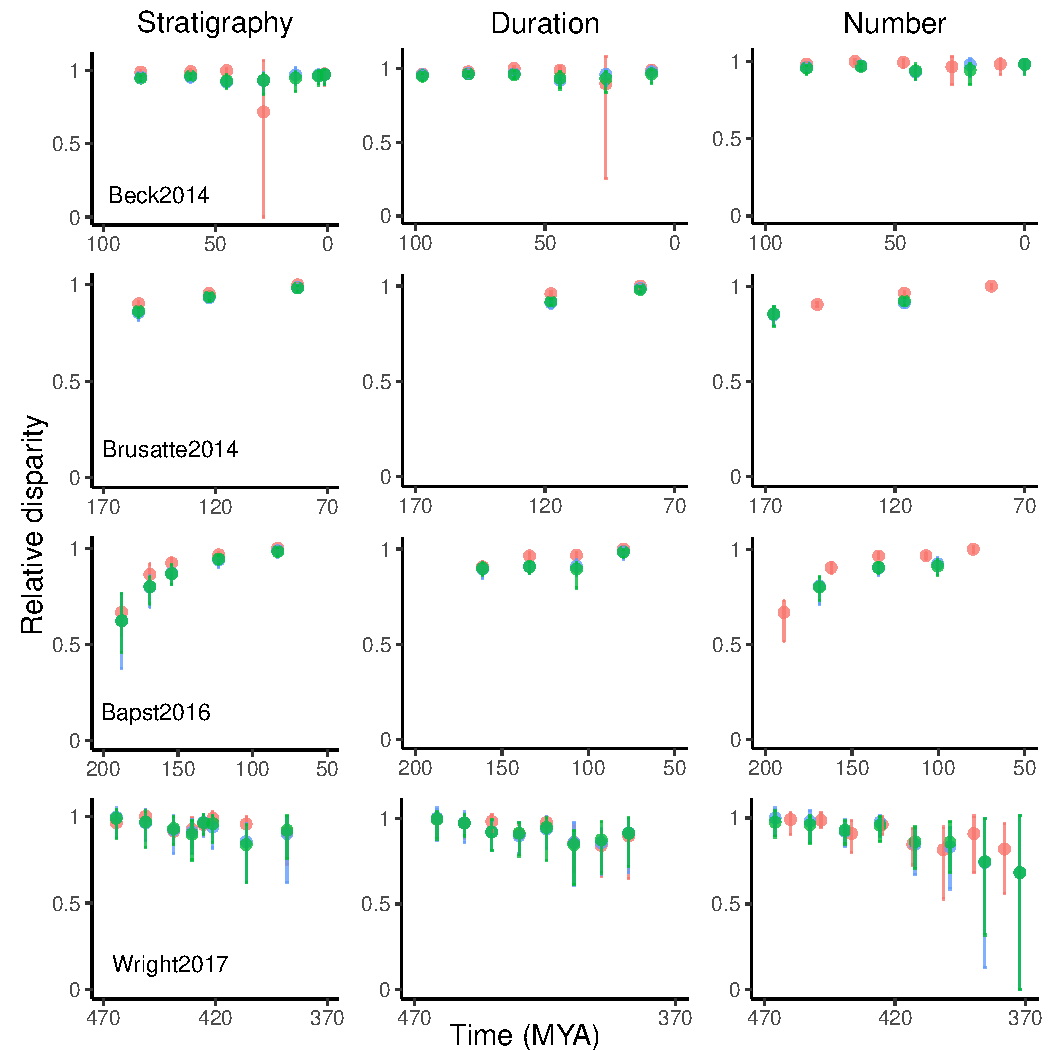
\includegraphics[width=1\linewidth, height=1\textheight, keepaspectratio]{figures/fig-dtt-epoch.pdf}
    \caption[Relative disparity through time for four example datasets.]
    {Median bootstrapped disparities were calculated using time binning and time-slicing approaches. 
    Pink points represent time binning methods, blue points are time slices with a punctuated model of evolution (specifically the `proximity' method), and green points are time slices with a gradual model of evolution (specifically the `gradual splits' method).
    Relative disparities (median bootstrapped disparity divided by the maximum median bootstrapped disparity for a dataset and analysis method) are presented so they can be compared across datasets/methods. 
    Stratigraphy uses unequal time bins or non-equidistant slices, where the width of the bin, or the interval between slices, is equivalent to stratigraphic epochs. 
    Duration uses equal time bins or equidistant slices, where the width of the bin, or the interval between slices, is the average duration of stratigraphic epochs in the time frame of the dataset. 
    Number uses equal time bins or equidistant slices, where the number of bins, or the number of slices, is the average number of stratigraphic epochs in the time frame of the dataset. 
    In all cases, time bin disparities are plotted at the midpoint of the bin, and error bars represent the 95\% confidence intervals around the bootstrapped median disparity.
    The four dataset names are on the first plot for each dataset (Table \ref{table:datasets}).
    Results for stratigraphic ages, and for other time-slicing models, are in the appendix.}
    \label{figure:dtt1}
  \end{figure}

\subsection{Testing for differences in the time sub-sampling methods}

\paragraph{Systematic differences in disparity-through-time.} 
There is no overall significant systematic difference among the disparities calculated using time bins and those calculated using the time-slicing methods. (Table \ref{table:wilcox}, Appendix Table \ref{table:wilcox2}). 
Instead, the differences depend on the dataset and method in question.
For example, the \cite{brusatte2014gradual}, \cite{bapst2016topology} and \cite{wright2017bayesian} datasets, show significant differences when using bins versus time slices defined by stratigraphy, but the \cite{beckancient2014} dataset appears robust to these different models.
Likewise, the \cite{beckancient2014}, \cite{brusatte2014gradual} and \cite{bapst2016topology} show different disparities when the number of bins or slices is the average number of stratigraphic periods, but this is not see in the \cite{wright2017bayesian} dataset.
Note that for epochs, we find fewer significant differences simply because the smaller numbers of bins and slices being compared means we have low power to detect a significant difference.

% Wilcoxon results table
%\begin{landscape}
  % latex table generated in R 3.4.2 by xtable 1.8-2 package
% Fri Dec  8 17:24:09 2017
\begin{table}[!htbp]
\caption{Results of paired Wilcoxon tests investigating whether disparities calculated using time bins are significantly different to those calculated using time-slices. Time-slices used either a  punctuated (‘proximity’ method) or gradual (‘gradual.split’ method) model of evolution. Stratigraphy uses unequal time bins or non-equidistant time-slices, where the width of the bin, or the interval between slices, is equivalent to stratigraphic ages or epochs. Duration uses equal time bins or equidistant time-slices, where the width of the bin, or the interval between slices, is the average duration of stratigraphic ages or epochs in the time frame of the dataset. Number uses equal time bins or equidistant time-slices, where the number of bins, or the number of slices, is the average number of stratigraphic ages or epochs in the time frame of the dataset. P-values were Bonferroni corrected. $***p < 0.001$. Results for other time-slicing methods are in the Supporting Information Appendix S2: Table A1.}
\centering
\begin{tabular}{lllccc}
  \hline
\textbf{Dataset} & \textbf{Period} & \textbf{Method} & \textbf{Stratigraphy} & \textbf{Duration} & \textbf{Number} \\ 
  \hline
  Beck2014 & Age & gradual.split & 111 & 115*** & 65*** \\ 
  Beck2014 & Age & proximity & 105 & 83 & 68*** \\ 
  Beck2014 & Epoch & gradual.split & 21 & 39 & 43*** \\ 
  Beck2014 & Epoch & proximity & 21 & 36 & 32 \\ 
  Brusatte2014 & Age & gradual.split & 28*** & 61*** & 52*** \\ 
  Brusatte2014 & Age & proximity & 27*** & 31 & 28*** \\ 
  Brusatte2014 & Epoch & gradual.split & 3 & 6 & 6 \\ 
  Brusatte2014 & Epoch & proximity & 0 & 5*** & 5 \\ 
  Bapst2016 & Age & gradual.split & 93 & 153 & 165 \\ 
  Bapst2016 & Age & proximity & 57*** & 47 & 75*** \\ 
  Bapst2016 & Epoch & gradual.split & 4 & 6 & 12 \\ 
  Bapst2016 & Epoch & proximity & 2 & 0*** & 8 \\ 
  Wright2017 & Age & gradual.split & 152*** & 155 & 116 \\ 
  Wright2017 & Age & proximity & 160*** & 175*** & 101 \\ 
  Wright2017 & Epoch & gradual.split & 28 & 29 & 21 \\ 
  Wright2017 & Epoch & proximity & 23 & 28 & 18 \\ 
   \hline
\end{tabular}

\label{table:wilcox} 
\end{table}
 
  \label{table:wilcox}  
%\end{landscape}

\paragraph{Disparity peaks and troughs.}
% Plots showing the differences

\paragraph{Effects of mass extinction events.}
% Big heat map table thing

%Fig. or Figs
%Fig width 80mm single column
%110mm - 2/3 width
%166mm full page

\section{Discussion}

Benefits of time slices

Further stuff to fix?



\section{Conclusions}
	

\section{Acknowledgments}
	NC thanks Mark Sutton and Phillip Mannion for the invitation to contribute to the `Evolutionary Modelling' symposium at The Palaeontological Association Annual Meeting 2017.
  TG acknowledges support from the Australian Discovery Project Grant number DP170103227 awarded to Vera Weisbecker.
  We thank Dave Bapst, Steve Brusatte, Graeme Lloyd, April Wright and Davey Wright for assistance in gathering data for the analyses.

\section{APPENDIX}

  \begin{figure}[!htbp]
    \centering
    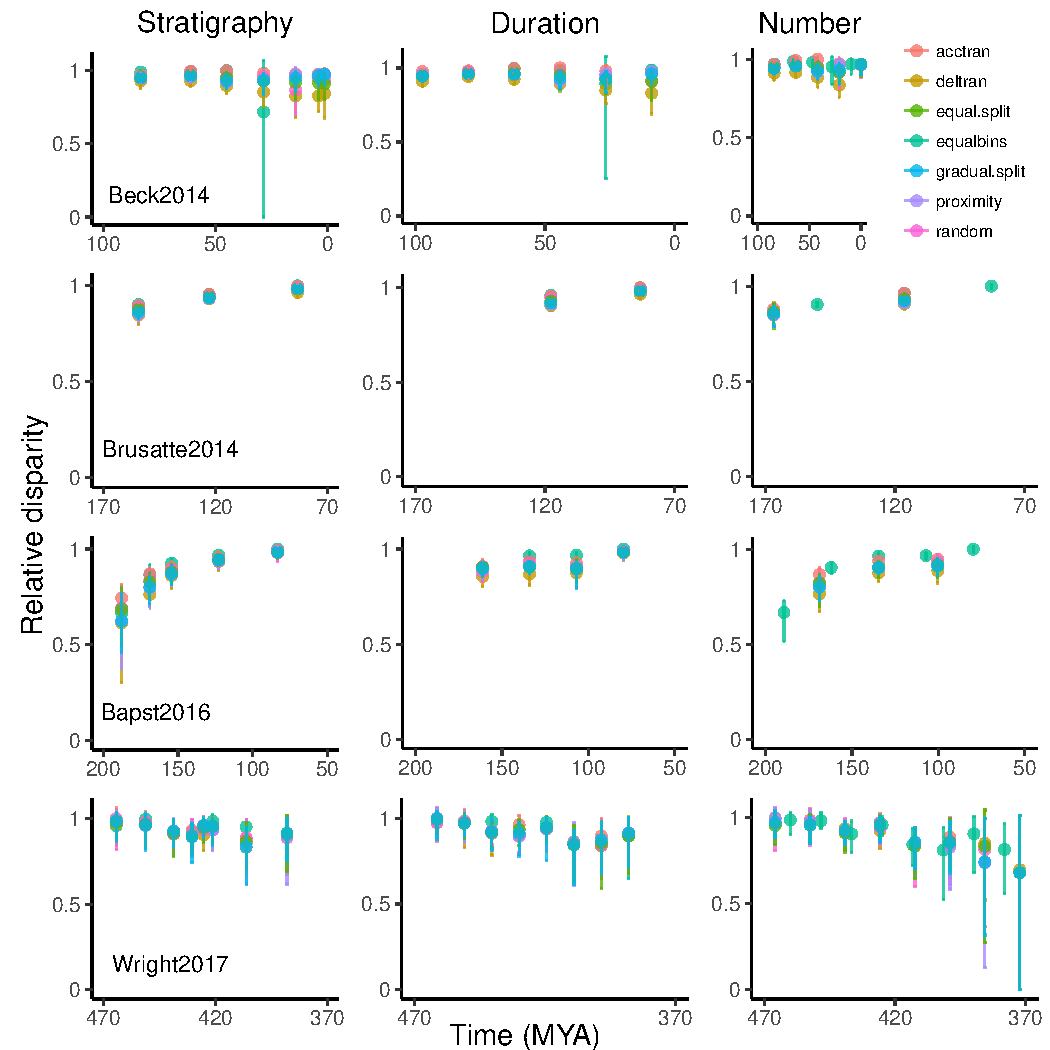
\includegraphics[width=1\linewidth, height=1\textheight, keepaspectratio]{figures/fig-dtt-epoch-appendix.pdf}
    \caption[Relative disparity through time for four example datasets.]
    {Median bootstrapped disparities were calculated using time binning and time-slicing approaches. 
    Pink points represent time binning methods, 
    % blue points are time slices with a punctuated model of evolution (specifically the `proximity' method), and green points are time slices with a gradual model of evolution (specifically the `gradual splits' method).
    Relative disparities (median bootstrapped disparity divided by the maximum median bootstrapped disparity for a dataset and analysis method) are presented so they can be compared across datasets/methods. 
    Stratigraphy uses unequal time bins or non-equidistant slices, where the width of the bin, or the interval between slices, is equivalent to stratigraphic epochs. 
    Duration uses equal time bins or equidistant slices, where the width of the bin, or the interval between slices, is the average duration of stratigraphic epochs in the time frame of the dataset. 
    Number uses equal time bins or equidistant slices, where the number of bins, or the number of slices, is the average number of stratigraphic epochs in the time frame of the dataset. 
    In all cases, time bin disparities are plotted at the midpoint of the bin, and error bars represent the 95\% confidence intervals around the bootstrapped median disparity.
    The four dataset names are on the first plot for each dataset (Table \ref{table:datasets}).}
    \label{figure:dtt2}
  \end{figure}  

  \begin{figure}[!htbp]
    \centering
    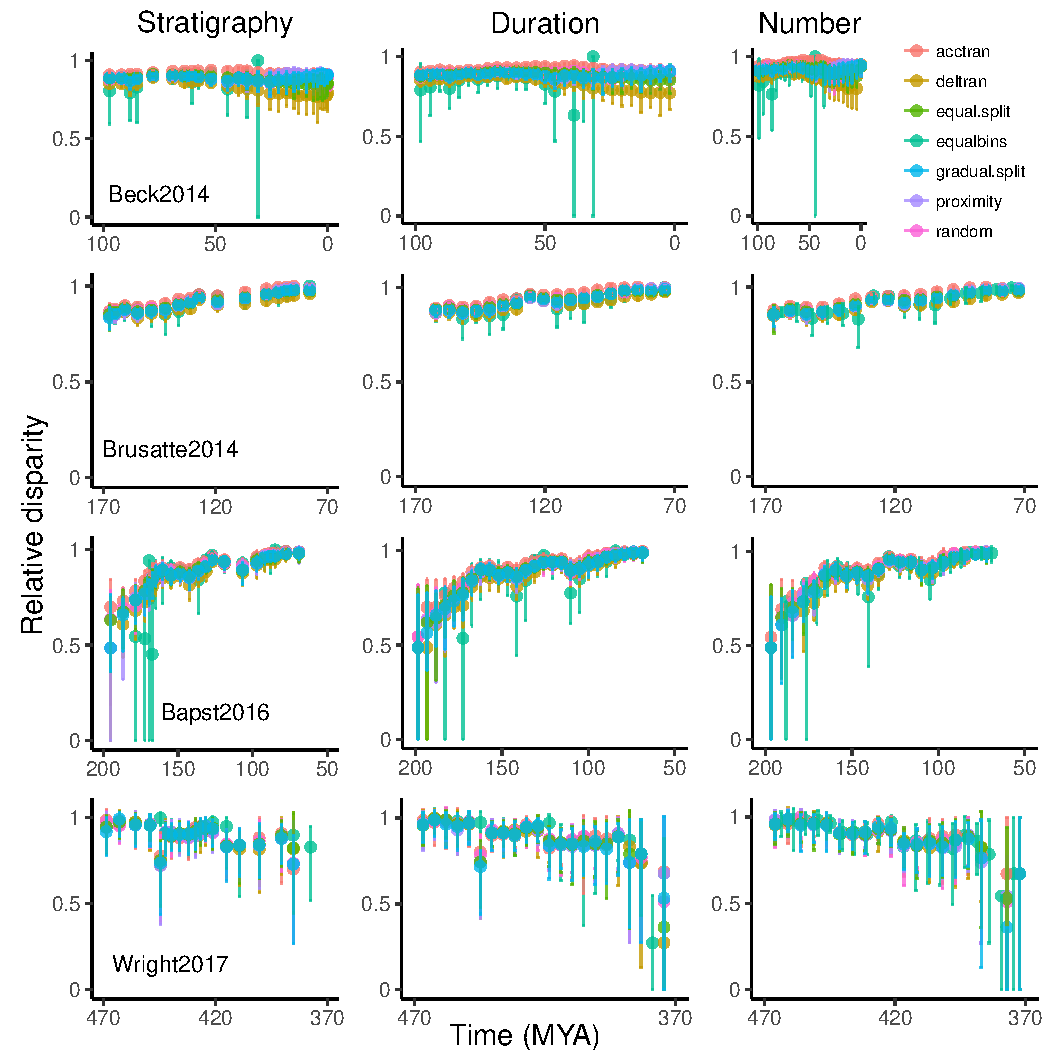
\includegraphics[width=1\linewidth, height=1\textheight, keepaspectratio]{figures/fig-dtt-age-appendix.pdf}
    \caption[Relative disparity through time for four example datasets.]
    {Median bootstrapped disparities were calculated using time binning and time-slicing approaches. 
    Pink points represent time binning methods, 
    %blue points are time slices with a punctuated model of evolution (specifically the `proximity' method), and green points are time slices with a gradual model of evolution (specifically the `gradual splits' method).
    Relative disparities (median bootstrapped disparity divided by the maximum median bootstrapped disparity for a dataset and analysis method) are presented so they can be compared across datasets/methods. 
    Stratigraphy uses unequal time bins or non-equidistant slices, where the width of the bin, or the interval between slices, is equivalent to stratigraphic ages. 
    Duration uses equal time bins or equidistant slices, where the width of the bin, or the interval between slices, is the average duration of stratigraphic ages in the time frame of the dataset. 
    Number uses equal time bins or equidistant slices, where the number of bins, or the number of slices, is the average number of stratigraphic ages in the time frame of the dataset. 
    In all cases, time bin disparities are plotted at the midpoint of the bin, and error bars represent the 95\% confidence intervals around the bootstrapped median disparity.
    The four dataset names are on the first plot for each dataset (Table \ref{table:datasets}).}
    \label{figure:dtt3}
  \end{figure}  

  % Wilcoxon results table
%\begin{landscape}
  % latex table generated in R 3.4.2 by xtable 1.8-2 package
% Fri Dec  8 17:06:33 2017
\begin{table}[!htbp]
\centering
\begin{tabular}{lllccc}
  \hline
\textbf{Dataset} & \textbf{Period} & \textbf{Model} & \textbf{Stratigraphy} & \textbf{Duration} & \textbf{Number} \\ 
  \hline
Beck2014 & Age & acctran & 39*** & 76 & 11 \\ 
  Beck2014 & Age & deltran & 188*** & 194*** & 171 \\ 
  Beck2014 & Age & equal.split & 91 & 119*** & 47 \\ 
  Beck2014 & Age & gradual.split & 111 & 115*** & 65*** \\ 
  Beck2014 & Age & proximity & 105 & 83 & 68*** \\ 
  Beck2014 & Age & random & 97 & 104*** & 45 \\ 
  Beck2014 & Epoch & acctran & 14 & 10 & 14 \\ 
  Beck2014 & Epoch & deltran & 21 & 45*** & 41*** \\ 
  Beck2014 & Epoch & equal.split & 21 & 40*** & 42*** \\ 
  Beck2014 & Epoch & gradual.split & 21 & 39 & 43*** \\ 
  Beck2014 & Epoch & proximity & 21 & 36 & 32 \\ 
  Beck2014 & Epoch & random & 21 & 37 & 45*** \\ 
  Brusatte2014 & Age & acctran & 27*** & 28 & 28*** \\ 
  Brusatte2014 & Age & deltran & 27*** & 29 & 31*** \\ 
  Brusatte2014 & Age & equal.split & 28*** & 58*** & 50*** \\ 
  Brusatte2014 & Age & gradual.split & 28*** & 61*** & 52*** \\ 
  Brusatte2014 & Age & proximity & 27*** & 31 & 28*** \\ 
  Brusatte2014 & Age & random & 27*** & 27 & 27*** \\ 
  Brusatte2014 & Epoch & acctran & 0 & 5*** & 5 \\ 
  Brusatte2014 & Epoch & deltran & 0 & 5*** & 5 \\ 
  Brusatte2014 & Epoch & equal.split & 3 & 6 & 6 \\ 
  Brusatte2014 & Epoch & gradual.split & 3 & 6 & 6 \\ 
  Brusatte2014 & Epoch & proximity & 0 & 5*** & 5 \\ 
  Brusatte2014 & Epoch & random & 0 & 5*** & 5 \\ 
  Bapst2016 & Age & acctran & 45*** & 47 & 72*** \\ 
  Bapst2016 & Age & deltran & 55*** & 46 & 78*** \\ 
  Bapst2016 & Age & equal.split & 93 & 147*** & 153 \\ 
  Bapst2016 & Age & gradual.split & 93 & 153 & 165 \\ 
  Bapst2016 & Age & proximity & 57*** & 47 & 75*** \\ 
  Bapst2016 & Age & random & 57*** & 48 & 81*** \\ 
  Bapst2016 & Epoch & acctran & 2 & 0*** & 8 \\ 
  Bapst2016 & Epoch & deltran & 2 & 0*** & 9 \\ 
  Bapst2016 & Epoch & equal.split & 4 & 6 & 13 \\ 
  Bapst2016 & Epoch & gradual.split & 4 & 6 & 12 \\ 
  Bapst2016 & Epoch & proximity & 2 & 0*** & 8 \\ 
  Bapst2016 & Epoch & random & 2 & 1*** & 8 \\ 
  Wright2017 & Age & acctran & 146*** & 146 & 84 \\ 
  Wright2017 & Age & deltran & 162*** & 138 & 101 \\ 
  Wright2017 & Age & equal.split & 151*** & 160 & 105 \\ 
  Wright2017 & Age & gradual.split & 152*** & 155 & 116 \\ 
  Wright2017 & Age & proximity & 160*** & 175*** & 101 \\ 
  Wright2017 & Age & random & 150*** & 147 & 111 \\ 
  Wright2017 & Epoch & acctran & 25 & 20 & 18 \\ 
  Wright2017 & Epoch & deltran & 27 & 26 & 25 \\ 
  Wright2017 & Epoch & equal.split & 29 & 30 & 25 \\ 
  Wright2017 & Epoch & gradual.split & 28 & 29 & 21 \\ 
  Wright2017 & Epoch & proximity & 23 & 28 & 18 \\ 
  Wright2017 & Epoch & random & 28 & 23 & 17 \\ 
   \hline
\end{tabular}
\caption{Wilcoxon results for appendix} 
\end{table}
 
  \label{table:wilcox2}  
%\end{landscape}
	
\bibliographystyle{palaeo} 
\bibliography{time-refs} 

\end{document}